\documentclass[aspectratio=169]{beamer}
\usepackage[UKenglish]{babel}
\usepackage[T1]{fontenc} % fontenc mit T1 sorgt für richtige Kodierung europäischer Zeichen
\usepackage[utf8]{inputenc} % Eingabezeichensatz: direkte Eingabe von Umlauten usw.
 % Anpassung des Dokumants deutsche Richtlinien

\usepackage{url} %Einbinden von Hyperlinks
\usepackage{mdwlist} % Für Listen ohne Abstand zwischen den Aufzählungspunkten.
\usepackage{paralist} % Ermöglicht Anpassung der Listen, z.B. Wahl des Autfählungszeichens

\usepackage{setspace} % Anpassung des Zeilenabstandes, Befehl muss vor der Berechnung des Satzspiegels gesetzt werden.

\usepackage{varioref} %Querverweise mit Seitenreferenz
\usepackage{fancyref} %Querverweise mit Angabe des Typs

\usepackage{xcolor}

%\usepackage[table,gray]{xcolor} %Zum Deaktivieren von Schattierung -- nur bei Verwendung des Packets "listings"
%\usepackage{listings} %Zur EInbindung von Quellcode verschiednester Art
\usepackage[locale=DE]{siunitx} % Korrekte Angabe von Einheiten
\usepackage[version=4]{mhchem}  % Für chemische Strukturformeln und Reaktionsgleichungen

\usepackage{booktabs} %Zur eleganten Formatierung von Tabellen
\usepackage{tabularx}
\usepackage{multirow} %Wenn man mehrere Zellen horizontal verbinden möchte
\usepackage[format = plain, textfont = normalfont, labelfont = bf, font = scriptsize, ]{caption}
%\usepackage[table,gray]{xcolor} %Zum Deaktivieren von Schattierung -- nur bei Verwendung des Packets "listings"
%\usepackage{listings} %Zur EInbindung von Quellcode verschiednester Art
%\usepackage[locale=DE]{siunitx} % Korrekte Angabe von Einheiten

\beamertemplatenavigationsymbolsempty

%\setbeamertemplate{footline}[text line]{%
%\parbox{\linewidth}{\vspace*{-8pt}Laser cooling\hfill\insertshortauthor\hfill\insertpagenumber}}

\useoutertheme{infolines}
\usecolortheme{beaver}

\title{F61: NMR--Spectroscopy}
%\subtitle{Seminarvortrag im Rahmen des Fortgeschrittenen-Praktikums}
\author{T. Gierlich und A. Impertro}
\date{}

\newcommand{\err}[2]{( #1 \, \pm \, #2 )}

\begin{document}

\begin{frame}
  \begin{center}
    {\LARGE F61: NMR--Spectroscopy}
    
    \bigskip
    
    {\large T. Gierlich and A. Impertro}
        
    \bigskip
   
    {\large May 26th, 2017}
  \end{center}
\end{frame}

\begin{frame}
	\frametitle{Outline}
  	\tableofcontents[subsubsectionstyle=hide]
\end{frame}

\section{Introduction and Theoretical Concepts}

\begin{frame}
	\frametitle{Introduction}
	\begin{figure}
		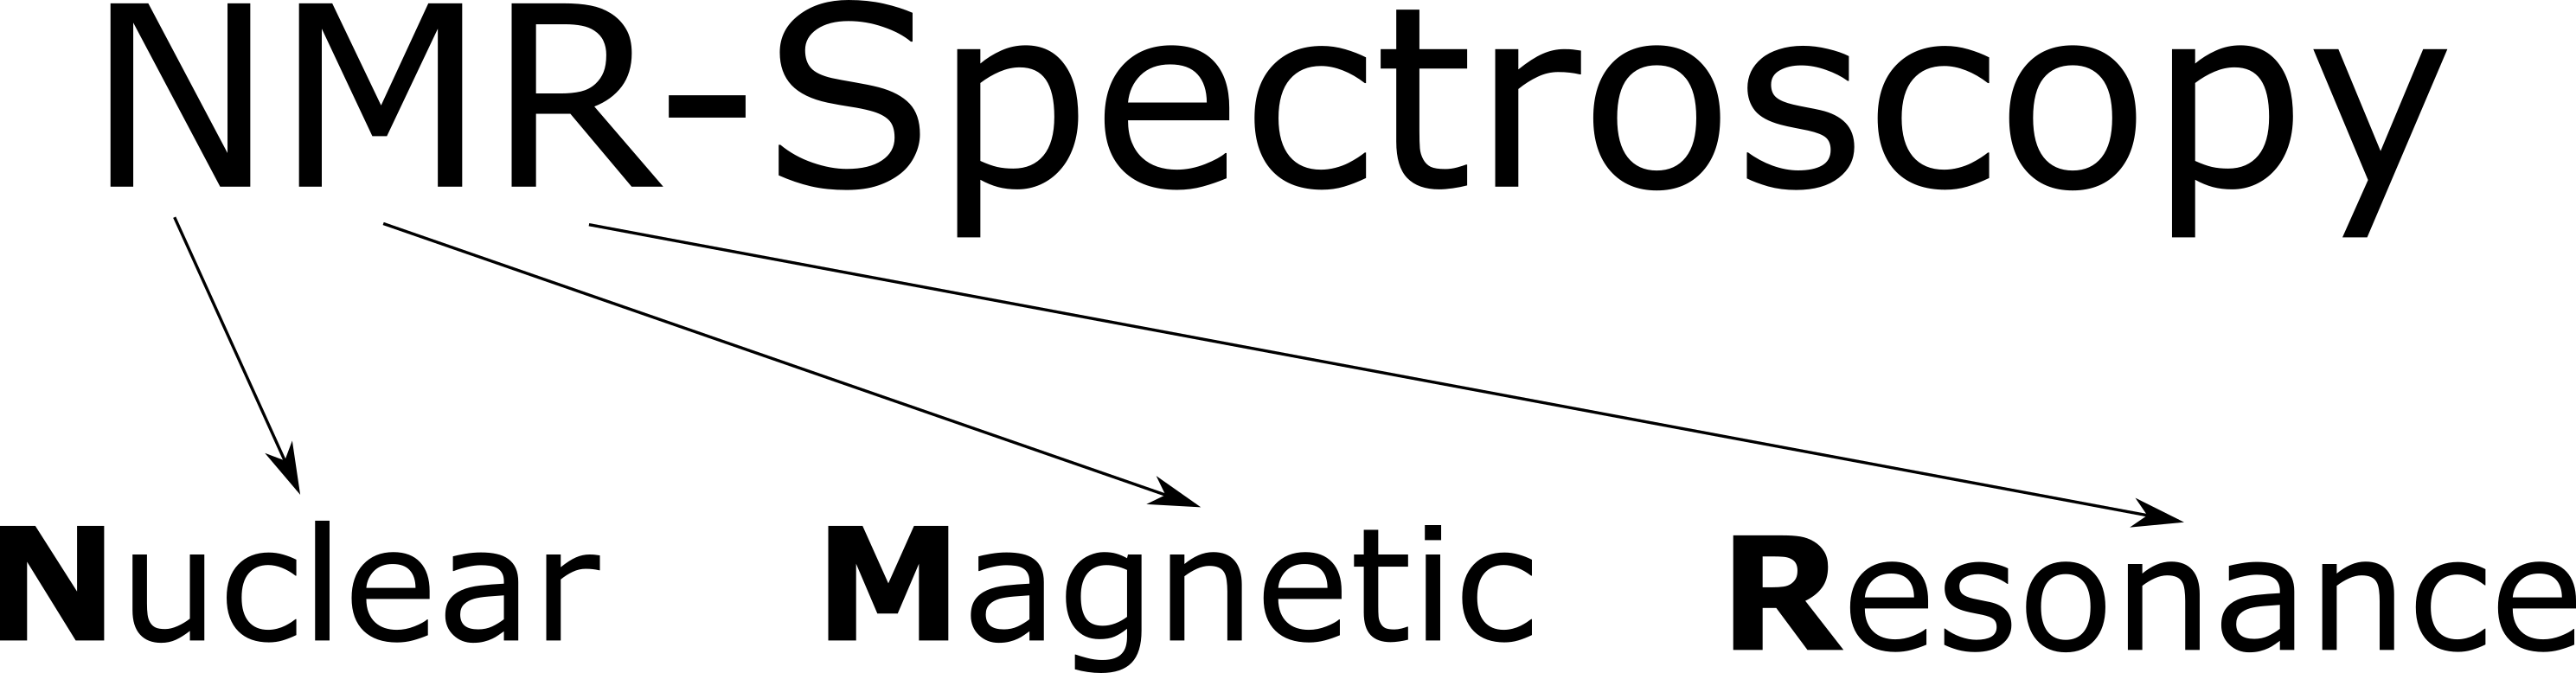
\includegraphics[width=0.5\textwidth]{./Resources/nmr_text.png}
		\label{fig:nmr_text}
	\end{figure}
	\flushleft
	%\begin{itemize}
	%	\item \textbf{Nuclear:} Interaction of the nuclear spin...
	%	\item \textbf{Magnetic:} ...with magnetic fields
	%	\item \textbf{Resonance:} $\rightarrow$ resonant interaction
	%	\item \textbf{Spectroscopy:} Resolve the different signal components
	%\end{itemize}
	\vspace*{-15pt}
	\pause
	\hrulefill
	\vspace*{5pt}
	%\textbf{Applications}
	
	\begin{minipage}[t]{0.48 \textwidth}
		\centering
		\textbf{Detection of substances}
		\begin{figure}
			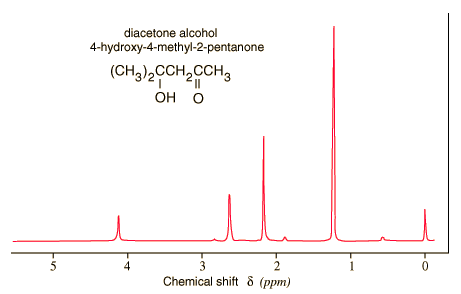
\includegraphics[height=0.3\textheight]{./Resources/cshift.png}
			\label{fig:cshift}
			\caption{\tiny{Carl Nave, Hyperphysics, hyperphysics.phy-astr.gsu.edu}}
		\end{figure}
	\end{minipage}
	\begin{minipage}[t]{0.48 \textwidth}
		\centering
		\textbf{Multidimensional imaging}
		\begin{figure}
			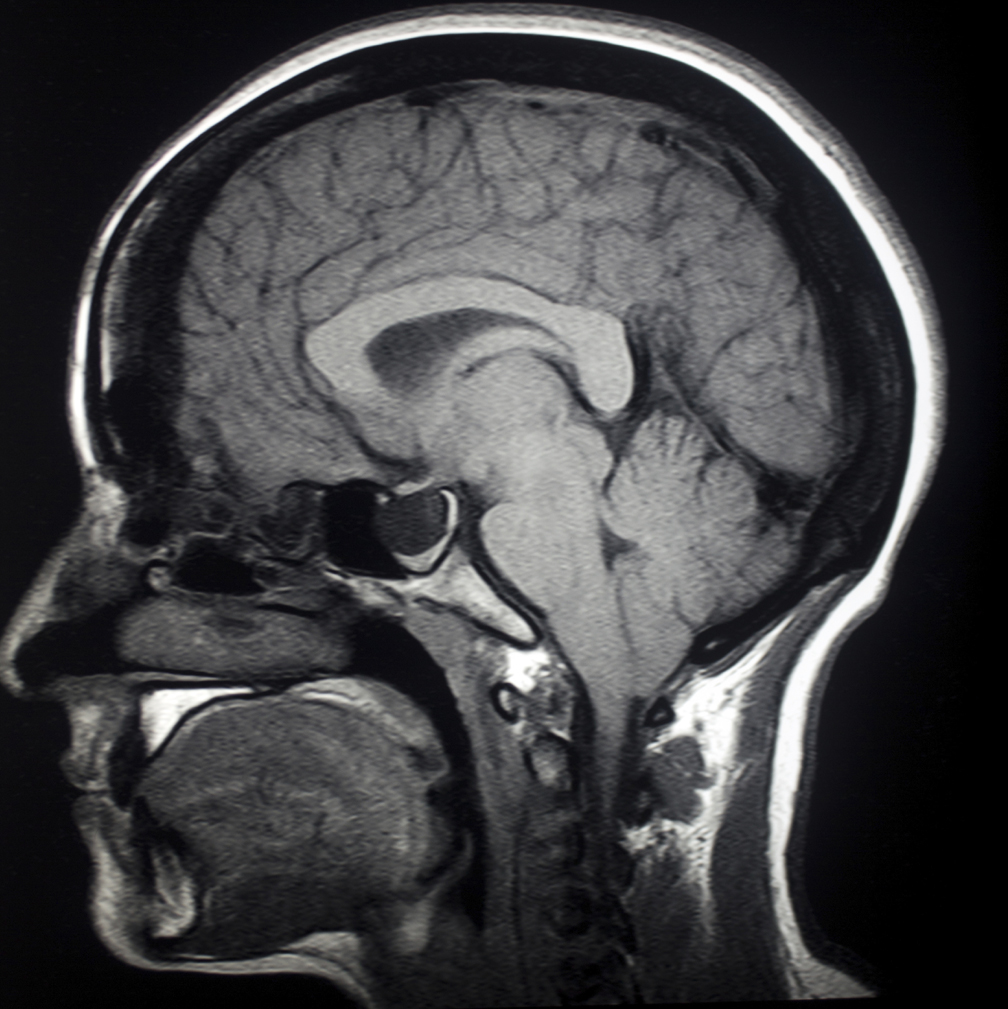
\includegraphics[height=0.3\textheight]{./Resources/mri_head.jpg}
			\label{fig:mri_head}
			\caption{\tiny{Sierra Vista Diagnostics, svdrads.com}}
		\end{figure}
	\end{minipage}
\end{frame}

\begin{frame}
	\frametitle{Theoretical Concepts - Working Principle}
	
	\begin{minipage}[t]{\textwidth}
		\begin{minipage}[t]{0.3\textwidth}
			\centering
			\begin{figure}
				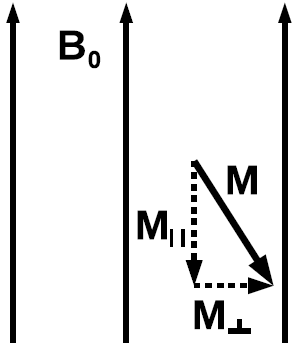
\includegraphics[height=0.3\textheight]{./Resources/magnetization_components.png}
				\caption{Magnetization}
				\label{fig:mag_components}
			\end{figure}
		\end{minipage}
		\begin{minipage}[t]{0.65\textwidth}
			\begin{itemize}
				\item Nuclei with spin $I$ have a magnetic moment $\mu$
				\item Ensemble of many nuclei: Measurable magnetization $\vec{M}$
				\item Minimal energy $\rightarrow$ Dipole aligned parallel to B-field
				\vspace{10pt}
				\item Ground state $\rightarrow$ $M_{\perp} = 0$
			\end{itemize}
			\vspace*{-5pt}
			\hrulefill
		\end{minipage}
	\end{minipage}
	\pause
	\begin{minipage}[t]{\textwidth}
		\begin{minipage}[t]{0.3\textwidth}
			\centering
			\begin{figure}
				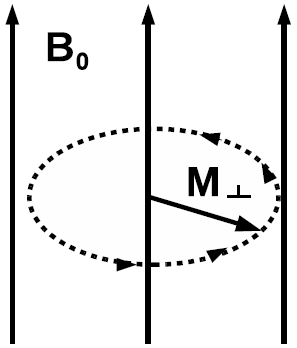
\includegraphics[height=0.3\textheight]{./Resources/larmor_precession.png}
				\caption{Larmor-Precession of $M_{\perp}$}
				\label{fig:larmor}
			\end{figure}
		\end{minipage}
		\begin{minipage}[t]{0.65\textwidth}
			\begin{itemize}
				\item Excited states have a component $M_{\perp} \neq 0$
				\item $M_{\perp}$ precesses around the field lines with the Larmor frequency
				\begin{equation}
					\omega_L = \gamma B_0
				\end{equation}
				\item $\omega_L$ can be measured!				
			\end{itemize}
		\end{minipage}
	\end{minipage}

\end{frame}

\begin{frame}
\frametitle{Theoretical Concepts - Working Principle}
\begin{minipage}[t]{0.65\textwidth}
	\textbf{How can we create an excited state ?}
	\begin{itemize}
		\item An oscillating B-Field $\vec{B}_1$ rotates the magnetization $\vec{M}$ by an angle
		\begin{equation}
		\alpha = \gamma B_1 \Delta t
		\end{equation}
	\end{itemize}
\end{minipage}
\hspace*{10pt}
\begin{minipage}[t]{0.3\textwidth}
	\begin{figure}[H]
		\centering
		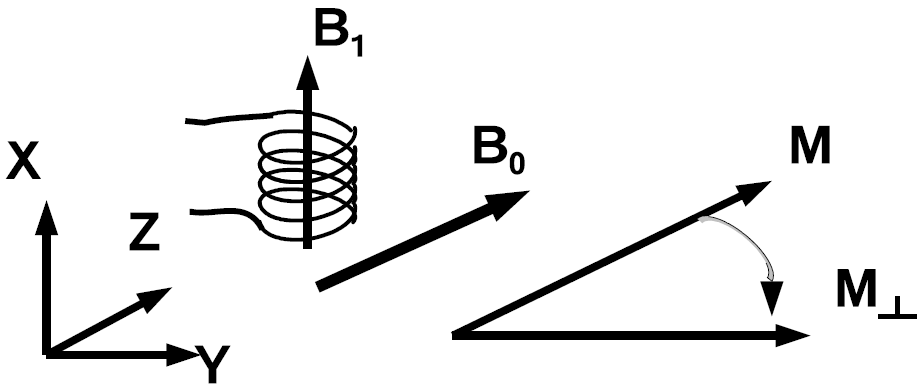
\includegraphics[width=\textwidth]{./Resources/hf_pulse.png}
		\caption{Rotation of $M$ due to an HF-Pulse}
	\end{figure}
\end{minipage}

\begin{itemize}
	\pause
	\item By choosing $\Delta t$, we can create:
	\begin{itemize}
		\item A perpendicular magnetization ($90^\circ$-Pulse)
		\item An anti-parallel magnetization ($180^\circ$-Pulse)
	\end{itemize}
\end{itemize}
\end{frame}

\begin{frame}
	\frametitle{Setup and Measurement Principle}
	\begin{figure}[H]
		\centering
		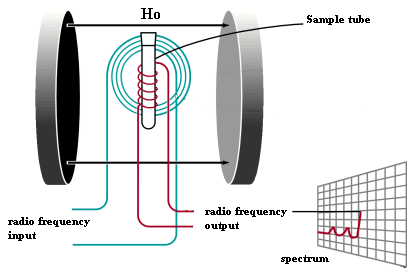
\includegraphics[height=0.7 \textheight]{./Resources/setup.png}
		\caption{\tiny{McGraw Hill Higher Education, mhhe.com}}
	\end{figure}
\end{frame}

\section{Part I: Relaxation Times}

\begin{frame}
	\frametitle{Theory of Relaxation}
	\textbf{Excited states decay into the Ground State on a characteristic timescale.}
	
	The decay is of exponential nature and described in the \textit{Bloch equations:}
	\begin{equation}
	\frac{dM_{\perp}(t)}{dt} = - \frac{M_{\perp}(t)}{T_2}
	\end{equation}
	\begin{equation}
	\frac{dM_{\parallel}(t)}{dt} = - \frac{M_{\parallel}(t) - M_0}{T_1}
	\end{equation}
	
	\begin{itemize}
		\item $T_2$: Spin-Lattice Relaxation
		\item $T_1$: Spin-Spin Relaxation
	\end{itemize}
\end{frame}

\begin{frame}
	\frametitle{$T_2$-Measurement: Spin Echo}
	\begin{minipage}[t]{0.45\textwidth}
		\centering
		\textbf{Spin-Echo principle}
		\begin{figure}
			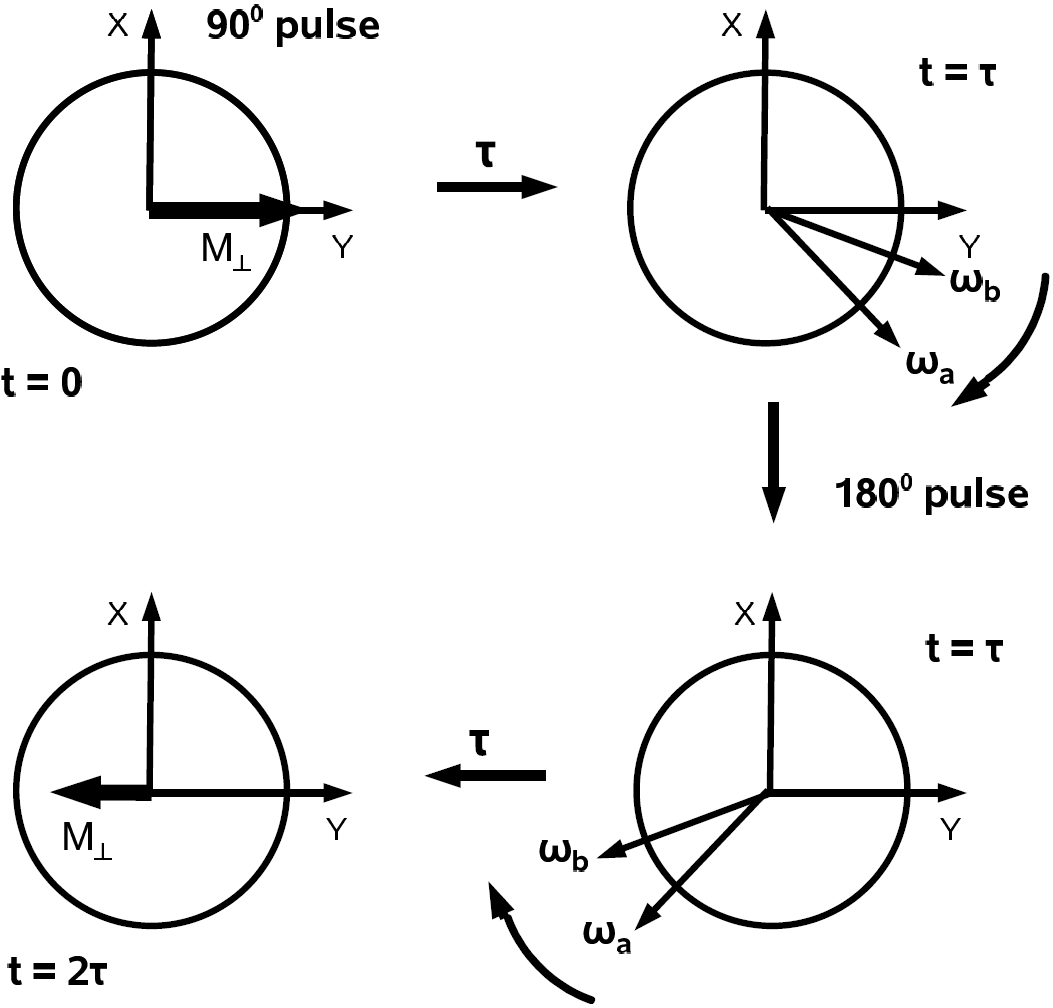
\includegraphics[height=40mm]{./Resources/spin_ech_schematic.png}
			\caption{Principle of the spin-echo method}
			\label{fig:spinecho_bloch}
		\end{figure}
	\end{minipage}
	\hfill
	\pause
	\begin{minipage}[t]{0.45\textwidth}
		\centering
		\textbf{Pulse sequence}
		\begin{figure}
			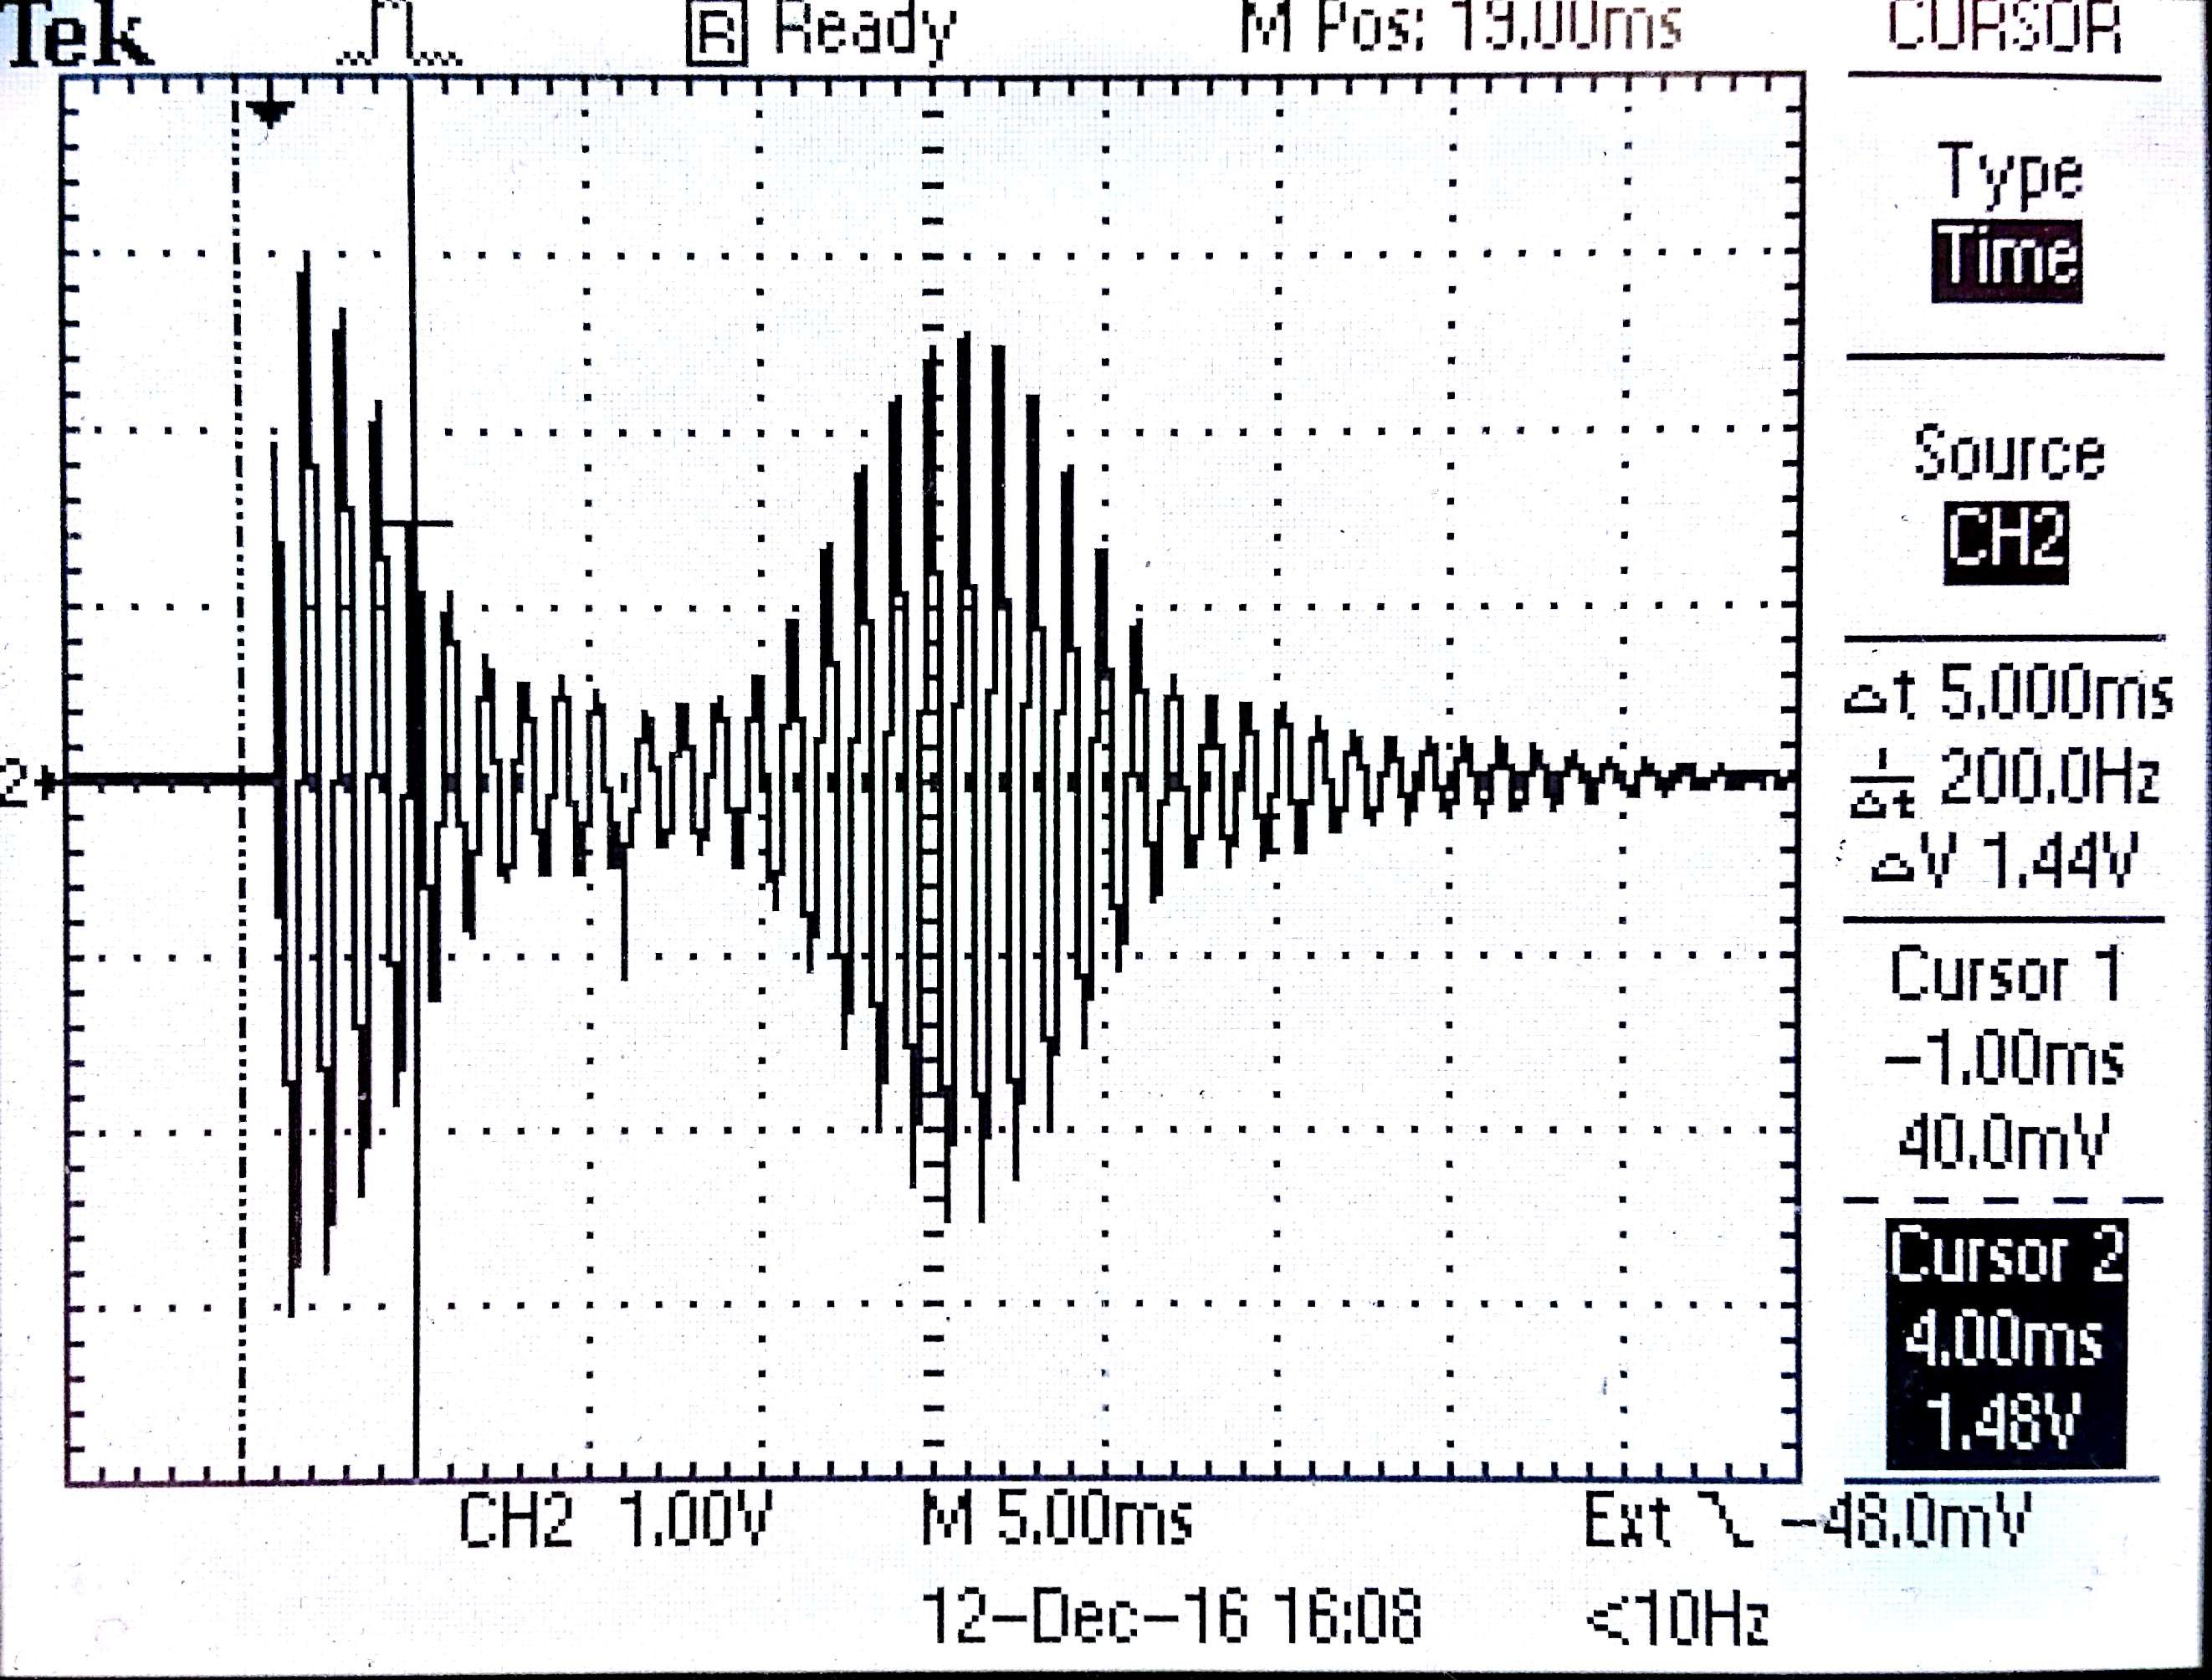
\includegraphics[height=40mm]{./Resources/spinecho_osci.jpg}
			\caption{Spin-Echo measurement with $\tau=10ms$}
			\label{fig:spinecho_osci}
		\end{figure}
	\end{minipage}
	\pause
	\begin{itemize}
		\item \textbf{Disadvantage}: Dephasing for long measurement times!
	\end{itemize}
\end{frame}

\begin{frame}
	\frametitle{$T_2$-Measurement: Spin Echo}
	\begin{minipage}[t]{0.45\textwidth}
		\centering
		\begin{figure}
			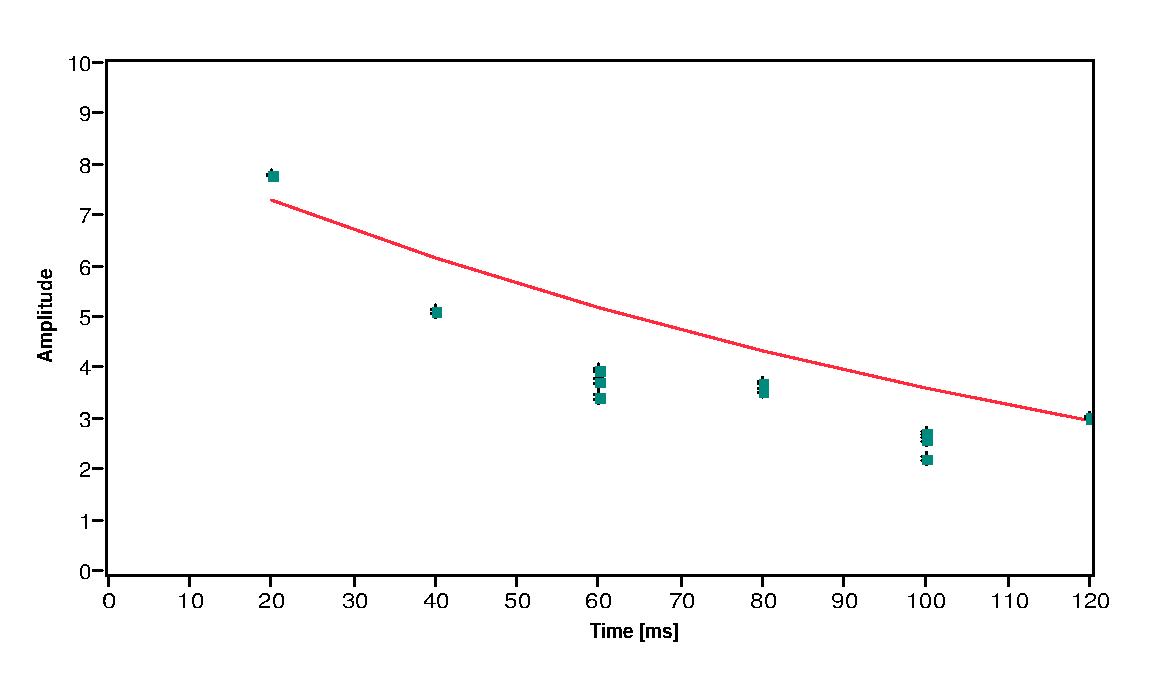
\includegraphics[width=70mm]{./Resources/t2_meas_p1.eps}
			\caption{T2-Measurement Sample 1 with fit.}
			\label{fig:t2_p1}
		\end{figure}
	\end{minipage}
	\hfill
	\begin{minipage}[t]{0.45\textwidth}
		\centering
		\begin{figure}
			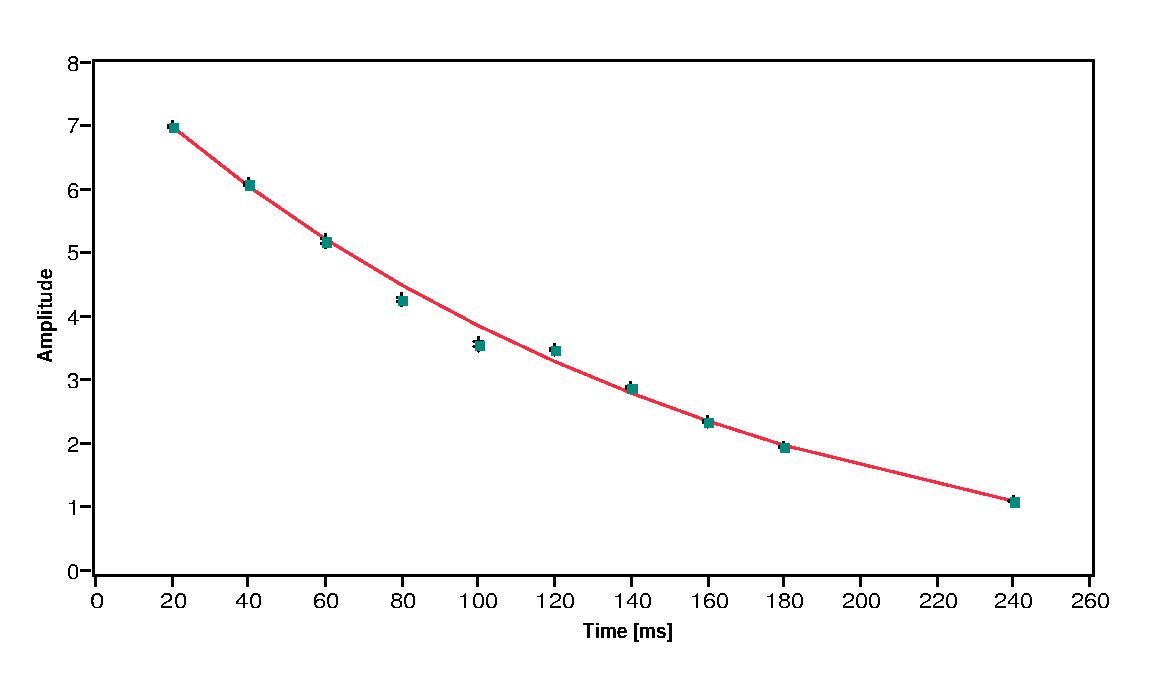
\includegraphics[width=70mm]{./Resources/t2_meas_p3.eps}
			\caption{T2-Measurement Sample 3 with fit.}
			\label{fig:t2_p3}
		\end{figure}
	\end{minipage}
\end{frame}

\begin{frame}
	\frametitle{$T_2$-Measurement: Carr-Purcell Sequence}
	\textbf{Improve dephasing problem of spin-echo method:}
	\begin{itemize}
		\item Inject a $180^\circ$-Pulse on odd multiples of a time $\tau$.
		\item The system is phase coherent on even multiples of a time $\tau$.
	\end{itemize}
	\pause
	\begin{minipage}[t]{0.45\textwidth}
		\centering
		\begin{figure}
			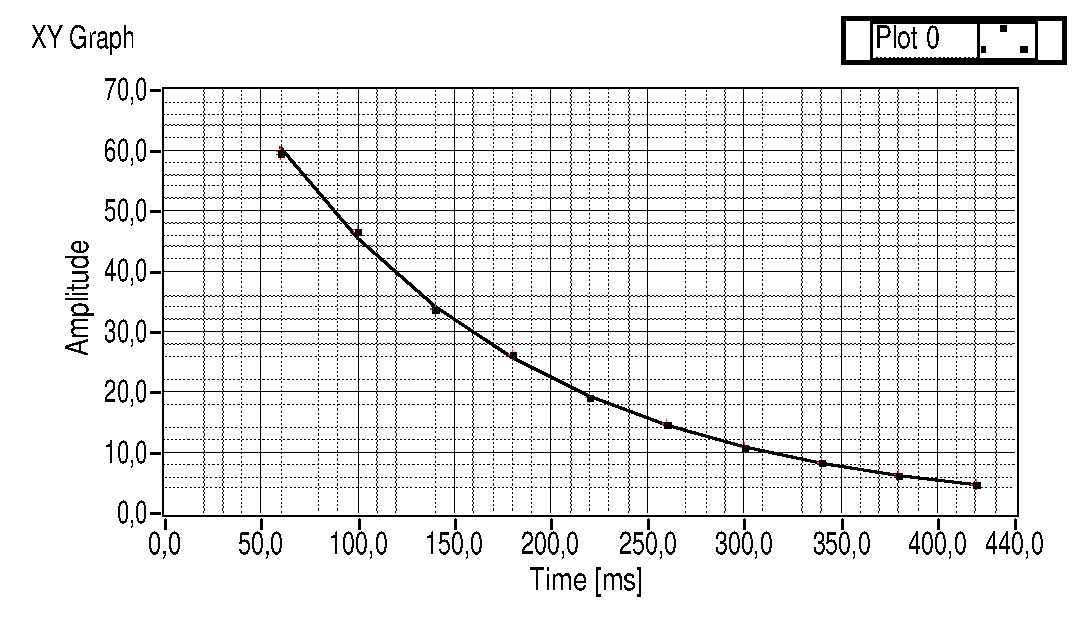
\includegraphics[width=60mm]{./Resources/t2_p1_cp.eps}
			\caption{T2-Measurement using Carr-Purcell, Sample 1, with fit.}
			\label{fig:t2_p1_cp}
		\end{figure}
	\end{minipage}
	\hfill
	\begin{minipage}[t]{0.45\textwidth}
		\centering
		\begin{figure}
			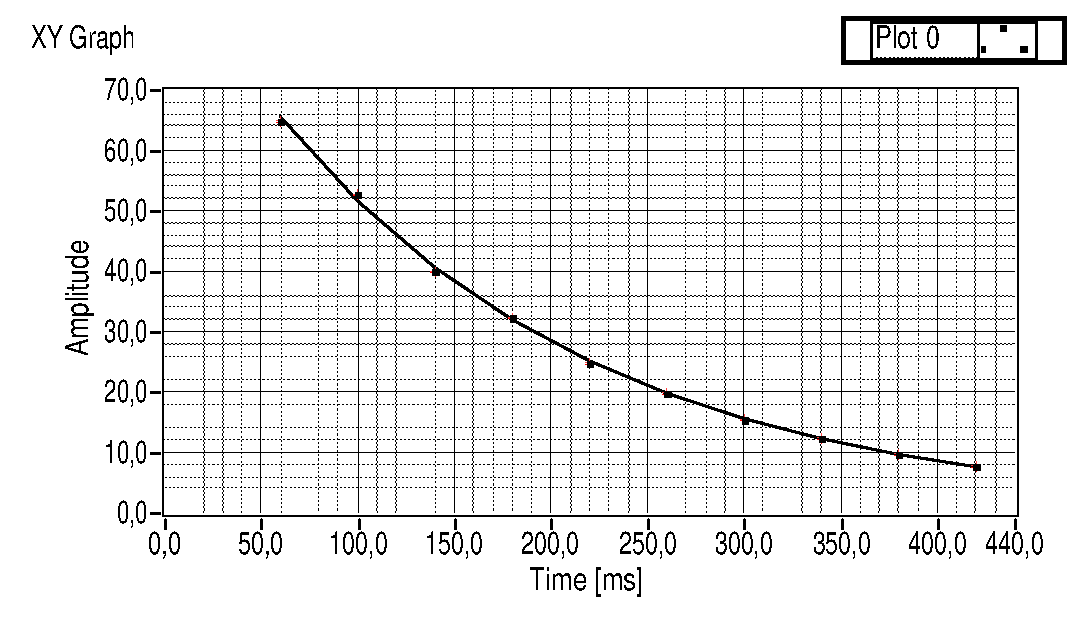
\includegraphics[width=60mm]{./Resources/t2_p3_cp.eps}
			\caption{T2-Measurement using Carr-Purcell, Sample 3, with fit.}
			\label{fig:t2_p3_cp}
		\end{figure}
	\end{minipage}
\end{frame}

\begin{frame}
	\frametitle{$T_1$-Measurement}
	\textbf{Start with a $180^\circ$-Pulse (Anti-parallel Magnetization) and probe the magnetization after time $\tau$ with a $90^\circ$-Pulse}
	
	\pause
	\begin{minipage}[t]{0.45\textwidth}
		\centering
		\begin{figure}
			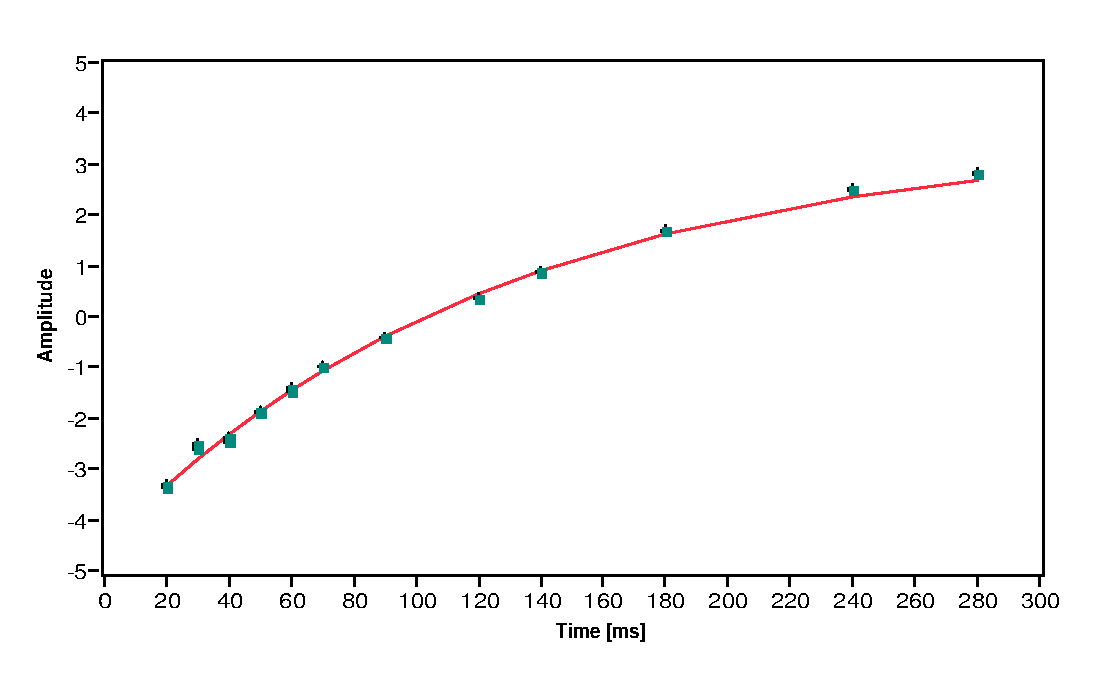
\includegraphics[width=60mm]{./Resources/t1_meas_p1.eps}
			\caption{T1-Measurement Sample 1 with fit.}
			\label{fig:t1_p1}
		\end{figure}
	\end{minipage}
	\hfill
	\begin{minipage}[t]{0.45\textwidth}
		\centering
		\begin{figure}
			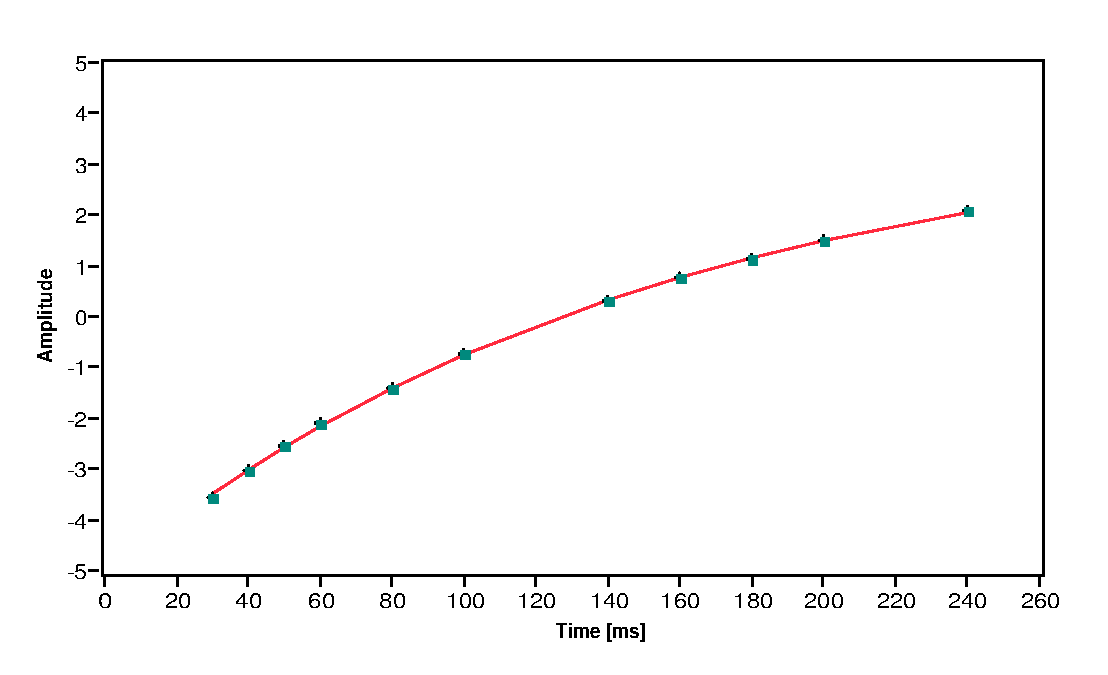
\includegraphics[width=60mm]{./Resources/t1_meas_p3.eps}
			\caption{T1-Measurement Sample 3 with fit.}
			\label{fig:t1_p3}
		\end{figure}
	\end{minipage}
\end{frame}

\begin{frame}
	\frametitle{Relaxation Times: Evaluation}
	\begin{table}[H] 
		\centering
		\caption{Relaxation times -- Measured values}
		\label{tab:relaxtimes}
		\begin{tabular}{cccc}
			\toprule
			Time & $T_1$ [$\mathrm{ms}$] & $T_2$ [$\mathrm{ms}$] & $T_2$ [$\mathrm{ms}$]\\
			Method & $180^\circ$-$90^\circ$ & Spin-Echo & Carr-Purcell\\
			\midrule
			Sample 1 (Gd 1:500)& $\err{125,5}{0,6}$ & $\err{119,5}{0,5}$ & $\err{140,1}{0,4}$\\
			Sample 3 (Gd 1:600)& $\err{150,5}{1,2}$ & $\err{139,3}{0,8}$ & $\err{166,9}{0,4}$\\
			\bottomrule
		\end{tabular}
	\end{table}
	
\end{frame}

\section{Part II. Chemical shift}

\subsection{Theory}

\begin{frame}
\frametitle{Chemical shift -- theory}
\begin{center}
	\textbf{Aim:} structure determination of chemical substances
\end{center}
\pause
\begin{columns}
	\column{.5\textwidth}
	\begin{itemize}
		\item electron orbitals contribute to $B_0$:
		\[\delta \vec{B} = \sigma \vec{B_0} \]
		\item modification of the Larmor frequency:
		\[ \omega_i = \omega_L \left(1-\sigma_i \right) \]
	\end{itemize}
	
	\column{.5\textwidth}
	\pause
	\begin{itemize}
		\item reference substance: TMS (Tetra-Methyl-Silan) 
		
		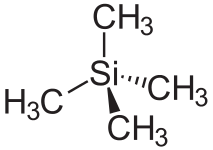
\includegraphics[width = 0.3\textwidth]{./Resources/Tetramethylsilan.png}
		\item relative chemical shift in ppm:
		\[ \delta_i = \sigma_i -\sigma_{TMS} = \frac{\omega_{TMS} - \omega_i}{\omega_L} \]
	\end{itemize}
\end{columns}
\end{frame}

\begin{frame}
\frametitle{Chemical shifts $\delta_i$ of compounds relative to TMS}

\begin{center}
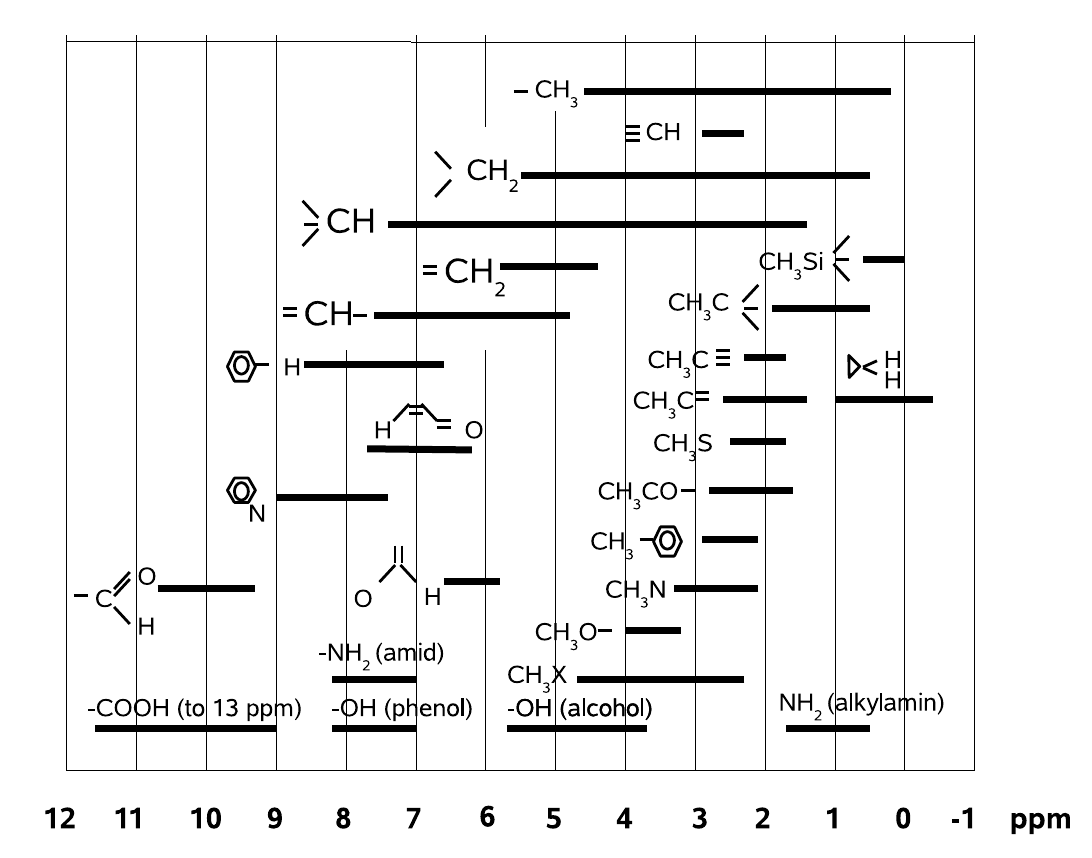
\includegraphics[width= 0.55\textwidth]{./Resources/chem_shifts.png}
\end{center}
\end{frame}

\subsection{Measurements}

\begin{frame}
\frametitle{Measurements}
\begin{itemize}
\item five chemical substances, with and without TMS
\item inhomogeneities and diffusion processes reduce resolution

$\Rightarrow$ thin glass tube, put into rotation with pressure air
\item result:
\begin{itemize}
\item without rotation: 

FWHM = \SI{200}{Hz}, I = 0,25
\item with rotation: 

FWHM = \SI{20}{Hz}, I = 1,9
\end{itemize}
\item energy resolution: 

$\Delta E_{NMR} = h \cdot \Delta \nu = 8,28 \cdot 10^{-14} \, \mathrm{eV}$
\end{itemize}
\end{frame}

\begin{frame}
\frametitle{Idenfication of the Probes}
\begin{center}
\textbf{Probe C: acetic acid} 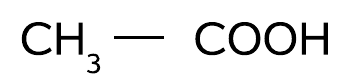
\includegraphics[height = 0.6 cm]{./Resources/acetic_acid.png}	
\end{center}

\begin{table}[!htb]
\centering
%\caption{Messergebnisse für Probe C, Zuordnung: \emph{Essigsäure} }
%\label{tab:Probe_C}
\begin{tabular}{cccl}
\toprule
Peaks of C+ [ppm] & Peaks of C [ppm] & Chem. shift. &  \\
\midrule
$p_1 = 16,7$ & $p_1 = 17,0$ & $\delta_i = 11,6$ & \ce{COOH}-group \\

$p_2 = 26,2$ & $p_2 = 26,6$ & $\delta_i = 2,1$ & Methyl group \ce{CH3} \\

$p_3 = 28,3$ & -- & -- & TMS \\
\bottomrule
\end{tabular}
\end{table}

\end{frame}

\begin{frame}
\frametitle{Idenfication of the Probes}
\begin{center}
\textbf{Probe B: p-Xylol} 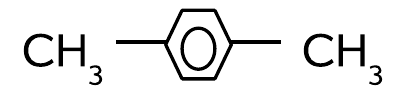
\includegraphics[height = 0.6 cm]{./Resources/p-xylol.png}
\end{center}

\begin{table}[!htb]
\centering
%\caption{Messergebnisse für Probe B, Zuordnung: \emph{p-Xylol} }
%\label{tab:Probe_B}
\begin{tabularx}{0.92\linewidth}{cccX}
\toprule
Peaks of B+ [ppm] & Peaks of B [ppm] & Chem. shift &  \\
\midrule
$p_1 = 22,7$ & $p_1 = 22,7$ & $\delta_i = 7,0$ & Benzene group \\

$p_2 = 27,5$ & $p_2 = 27,5$ & $\delta_i = 2,2$ & Methyl group, Peak twice as high as $p_1$ \\

$p_3 = 29,7$ & -- & --  & TMS \\

\bottomrule
\end{tabularx}
\end{table}	

\end{frame}

\begin{frame}
\frametitle{Idenfication of the Probes}
\begin{center}
\textbf{Probe E: toluol} 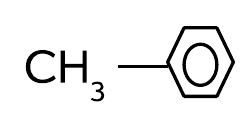
\includegraphics[height = 0.6 cm]{./Resources/toluol.png}
\end{center}

\begin{table}[!htb]
\centering
%	\caption{Messergebnisse für Probe E, Zuordnung: \emph{Toluol} }
%	\label{tab:Probe_E}
\begin{tabularx}{.92\linewidth}{cccX}
\toprule
Peaks of E+ [ppm] & Peaks of E [ppm] & Chem. shift &  \\
\midrule
$p_1 = 19,5$ & $p_1 = 23,1$ & $\delta_i = 7,3 $ & Benzene group \\

$p_2 = 24,4$ & $p_2 = 23,1$ & $\delta_i = 2,4$ & Methyl group, peaks have same hight \\

$p_3 = 26,8$ & -- & -- & TMS \\

\bottomrule
\end{tabularx}
\end{table}

\end{frame}



\begin{frame}
\frametitle{Idenfication of the Probes}
\begin{center}
\textbf{Probe A: fluoroaceton} 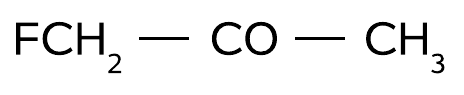
\includegraphics[height = 0.6 cm]{./Resources/fluoroacetone.png}
\end{center}

\begin{table}[!htb]
\centering
%\caption{Messergebnisse für Probe A, Zuordnung: \emph{Flouraceton} }
%\label{tab:Probe_A}
\begin{tabularx}{.90\linewidth}{cccX}
\toprule
Peaks of A+ [ppm] & Peaks of A [ppm] & Chem. shift &  \\
\midrule
$p_1 = 22,2$ & $p_1 = 23,8$ & $\delta_i = 6,3$ & \multirow{2}{*}{\ce{FCH2}-group} \\

$p_2 = 24,6$ & $p_2 = 21,4$ & $\delta_i= 3,9$ &  \\

$p_3 = 26,4$ & $p_3 = 19,6$ & $\delta_i = 2,1 $ & Methyl group \ce{CH3} \\

$p_4 = 28,5$ & -- & -- & TMS \\
\bottomrule
\end{tabularx}
\end{table}

\end{frame}

\begin{frame}
\frametitle{Idenfication of the Probes}
\begin{center}
\textbf{Probe D: fluoroacetonitril} 
\includegraphics[height = 0.6 cm]{./Resources/fluoroacetonitril.png}
\end{center}

\begin{table}[!htb]
\centering
%	\caption{Messergebnisse für Probe D, Zuordnung: \emph{Fluoroacetonitril} }
%	\label{tab:Probe_D}
\begin{tabularx}{.9\linewidth}{cccX}
\toprule
Peaks of D+ [ppm] & Peaks of D [ppm] & Chem. shift &  \\
\midrule
$p_1 = 30,8$ & -- & -- & TMS \\

$p_2 = 34,8$ & $p_2 = 26,6$ & $\delta_i = 6,4$ & \multirow{2}{*}{\ce{FCH2} group} \\

$p_3 = 37,2$ & $p_3 = 24,2$ & $delta_i = 4,0$ &  \\

\bottomrule
\end{tabularx}
\end{table}
\end{frame}

\section{Imaging with NMR}

\subsection{Theory}

\subsubsection{one dimensional imaging}

\begin{frame}
\frametitle{one dimensional imaging -- theory}
\begin{itemize}
\item \textbf{position dependent magnet fields}
\item Superposition of the static field $\vec{B_0}$ with gradient fields $\vec{B^x}$, $\vec{B^y}$, $\vec{B^z}$
\item two techniques:
\end{itemize}
\begin{columns}
\column{.5\textwidth}
\begin{description}
\item[frequency coding]
\end{description}
\begin{itemize}
\item Larmor frequency $\omega_L = \gamma (B_0 + G^z \cdot z) = \omega_L^0 + \omega_z$
\item measured NMR signal $S(t)$ is Fourier transform of $M_{\perp}^{rot}(z)$
\end{itemize}
\column{.5\textwidth}
\begin{description}
\item[phase coding]
\end{description}
\begin{itemize}
\item apply gradient field, increase strength
\item phase rotates: $\phi (z) = (\gamma G^z T_{Ph})z = k_z z$
\end{itemize}

\end{columns}	
\end{frame}

\begin{frame}
\frametitle{two dimensional imaging -- theory}
\begin{center}
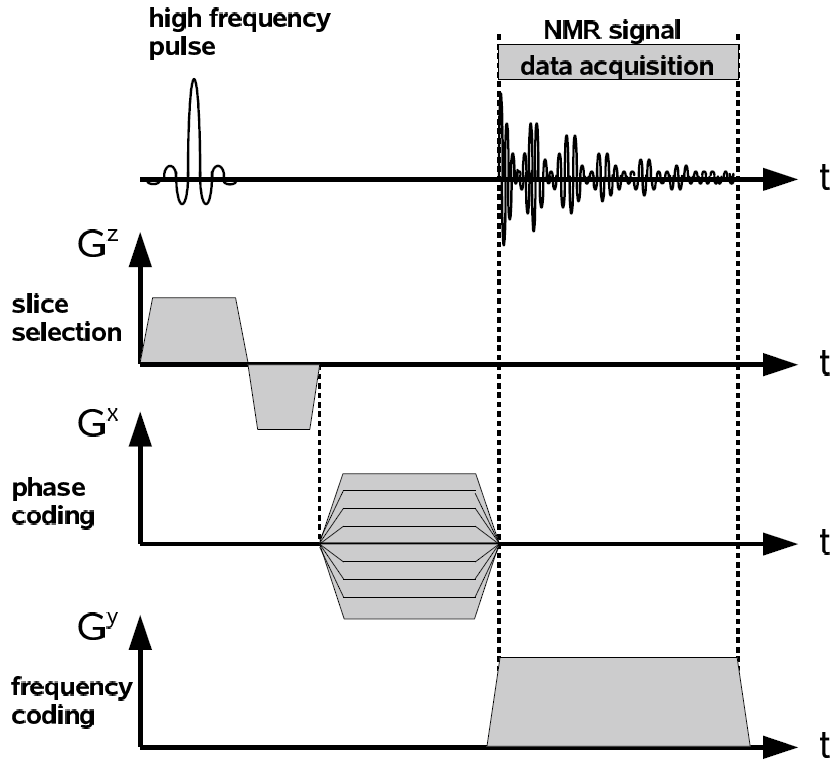
\includegraphics[width=0.4\linewidth]{./Resources/2d_imaging.png}
\end{center}

\end{frame}

\subsection{Experiments}

\subsubsection{one dimensional imaging}

\begin{frame}
\frametitle{One dimensional imaging measurements}
\begin{columns}
\column{.5\textwidth}
\begin{itemize}
\item Bruker$^{\textregistered}$ NMR analyzer mq7.5
\item Glass tube filled with \SI{15}{mm} of oil
\item Glass tube filled with \SI{50}{mm} of water
\item glass tube with teflon structure
\item examination of an inflitration process: 

Fick's second law: $\frac{\partial c}{\partial t} = D \frac{\partial^2 c}{\partial x^2}$
\end{itemize}

\column{.5\textwidth}
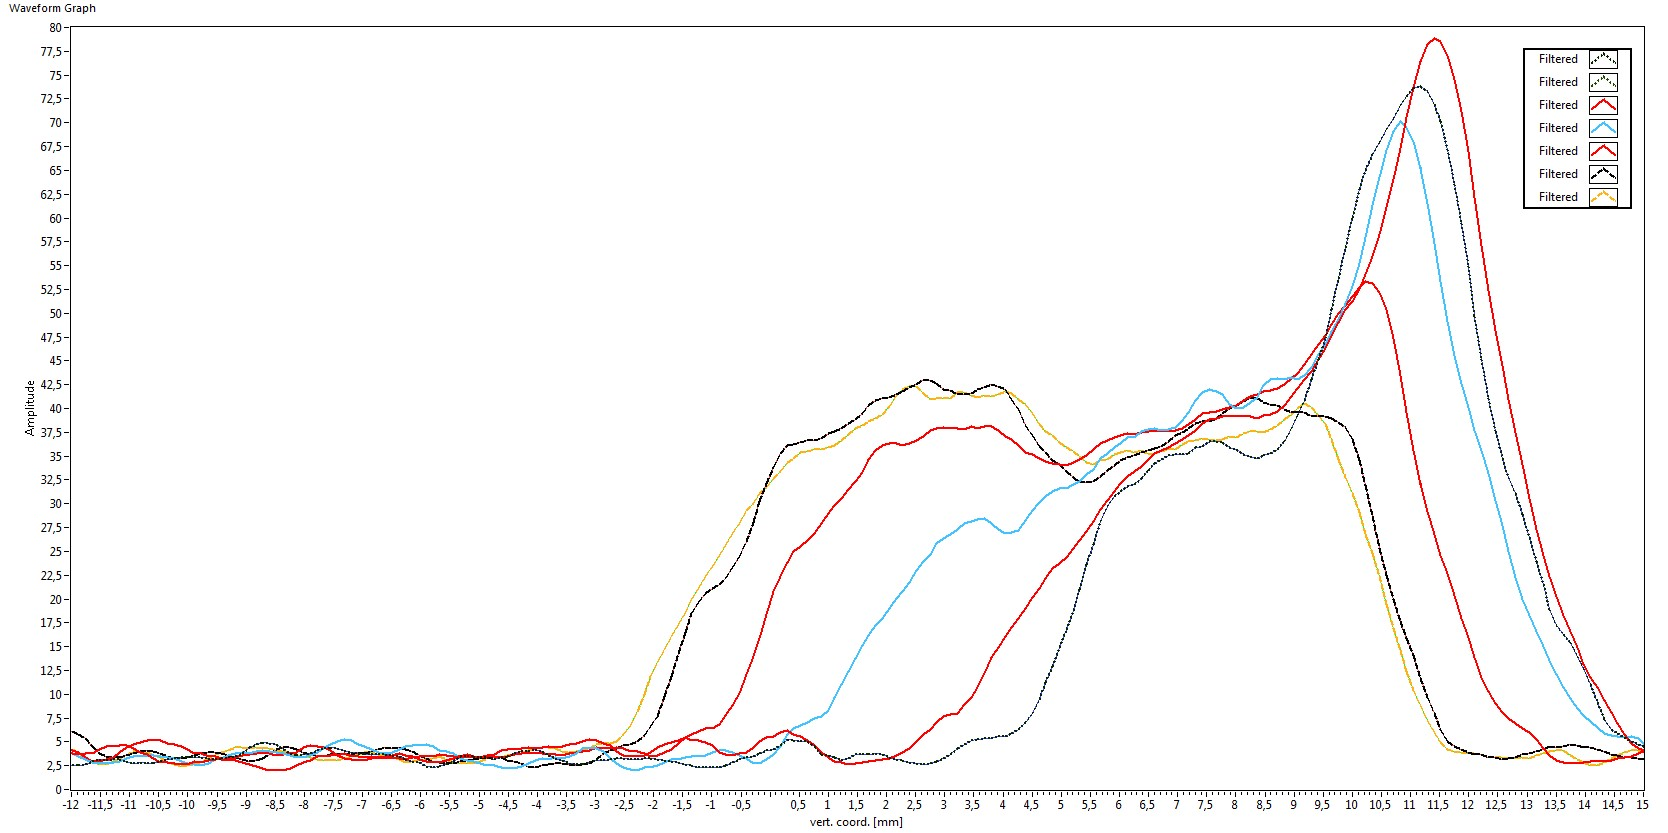
\includegraphics[width=1.0 \linewidth]{./Resources/Teil_3/oeldiff_chinchilla.jpg}
\end{columns}	
\end{frame}

\subsubsection{two dimensional imaging}

\begin{frame}
\frametitle{two dimensional imaging measurements}
\begin{columns}
\column{.5\textwidth}
\begin{figure}
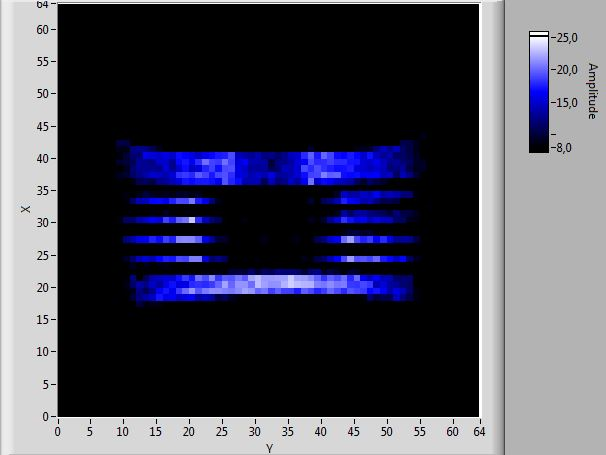
\includegraphics[width=.80 \linewidth]{./Resources/Teil_3/ptfe_vert.JPG}
\caption{teflon structure}
\end{figure}

\column{.5\textwidth}
\begin{figure}
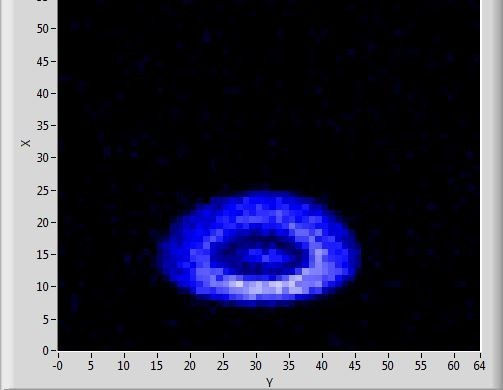
\includegraphics[width=0.8 \linewidth]{./Resources/Teil_3/olive_2d.JPG}
\caption{olive}
\end{figure}

\end{columns}
\end{frame}

\begin{frame}
\frametitle{two dimensional imaging measurements}
\begin{columns}
\column{.5\textwidth}
\begin{figure}
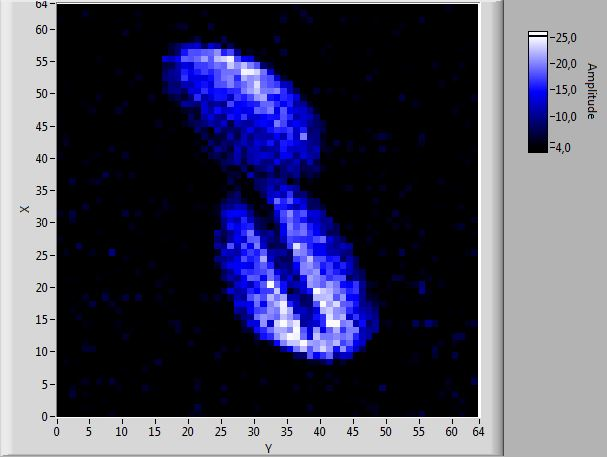
\includegraphics[width=.80 \linewidth]{./Resources/Teil_3/peanut_shell.JPG}
\caption{peanut shell}
\end{figure}

\column{.5\textwidth}
\begin{figure}
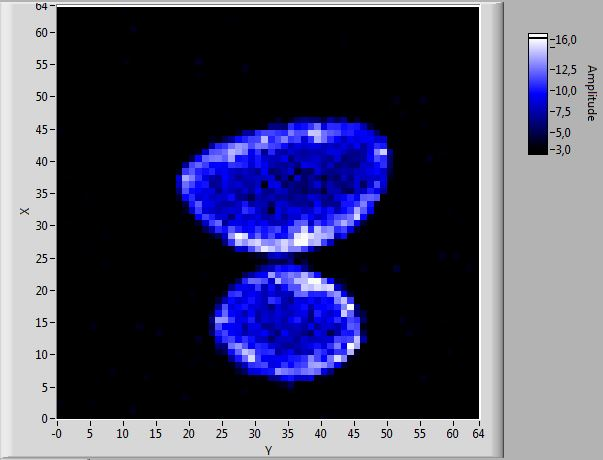
\includegraphics[width=0.8 \linewidth]{./Resources/Teil_3/aloevera_2d.JPG}
\caption{aloe vera}
\end{figure}

\end{columns}
\end{frame}

\end{document}